\chapter{Background}

\section{Fundamental Walking Dynamics}
\subsection{Rimless wheel}
\subsection{Inverted Pendulum}
\subsection{Bipedal Spring Mass}

\section{Walking Controls}

Shaping walking Dynamics through control
\subsection{Kinematic Centralized Controllers}

These approaches are usually model based and try to force the full system to
behave like a lower dimensional system. We can derive provably stable
controllers for lower order systems so if full order system behaves like lower
order system it will not fall.


    \begin{itemize}
        \item ZMP preview control - forces robot to follow kinematics of lipm
        model
    \end{itemize}

\subsection{Dynamic Centralized Controllers}
    Force control allows robots to be compliant to external disturbances.

    \begin{itemize}
        \item Model reduction approaches:        
            \begin{itemize}
                \item DRC  QP controllers force robots to follow dynamics of
                    point mass systems
                \begin{itemize}
                    \item Gaits are still statically stable
                    \item dynamic in the sense that these controllers command forces
                        not kinematics
                \end{itemize}


                \item Spring mass model similar to previous approaches but force
                the robot to follow the dynamics of spring mass model

                \item Hybrid zero dynamics for full robots reduce dynamics to
                those of a single degree of freedom theo jansen walker
            \end{itemize}

        \item Heuristic Centralized/dynamic approaches
        \begin{itemize}
            \item Neural Network Dog controller - high level centralized neural
            network for commanding parameters of decentralized lower-level
            impedance controllers
        \end{itemize}
    \end{itemize}

Centralized controllers rely heavily on models causes two problems
\begin{enumerate}
    \item QPs and inverse dynamics result in unnatural, inneficient gaits to avoid
    singularity which causes
    \item Its unlikely we can model the diverse population of amputees in order
    to derive centralized controllers that consider the joint amputee/prosthesis
    dynamics.
\end{enumerate}
This motivates alternative heuristic decentralized controllers.


\subsection{Kinematic Decentralized Controllers}
    \begin{itemize}
        \item echo control
    \end{itemize}
\subsection{Dynamic Decentralized Controllers}
    \begin{itemize}
        \item raibert - motivation for landing leg angles
        \item virtual model control

        \item Applicable to prostheses
        \begin{itemize}
            \item not bio inspired
                \begin{itemize}
                    \item simbicon/impedance control
                    \item hybrid zero dynamics for prostheses
                \end{itemize}

            \item bio inspired

                We can derive another class of dynamic, decentralized
                controllers from biological models of animal and human
                locomotion. These models simulate locomotion at the level of the
                central nervous system, through simplified models of neural
                circuitry. 
                \begin{description}
                    \item[Central Pattern Generators (CPGs)]
                        
                    \item[neuromuscular model] 
                \end{description}
        \end{itemize}
   \end{itemize}

\subsubsection{Central Pattern Generators}
Central Pattern Generators (CPGs) are hypothesized nonlinear
oscillators, comprised of neurons in the central nervous system, that can
autonomously generate periodic neural activation
patterns~\citep{ijspeert2008central}.  \citet{brown1911intrinsic} first
suggested their existence based on experiments he conducted on decerebrated and
deafferented cats. In these experiments, \citeauthor{brown1911intrinsic} severed
both the afferent pathways (that carry sensory information) and efferent
pathways (that transmit higher level commands from the brain to motor neurons).
Despite the lack of high level control and sensory feedback, the cats still
displayed cyclical motions in their hind legs similar to those seen during
normal gait. This result suggests CPGs may play an important role in generating
locomotion controls in vertebrate animals. Similar cyclical neural activity
(called fictive locomotion) has been found in isolated lamprey spinal cords
\citep{cohen1980neuronal}, salamanders \citep{delvolve1999fictive}, and frog
embryos \citep{soffe1982tonic}. 

\begin{marginfigure}
    \centering
    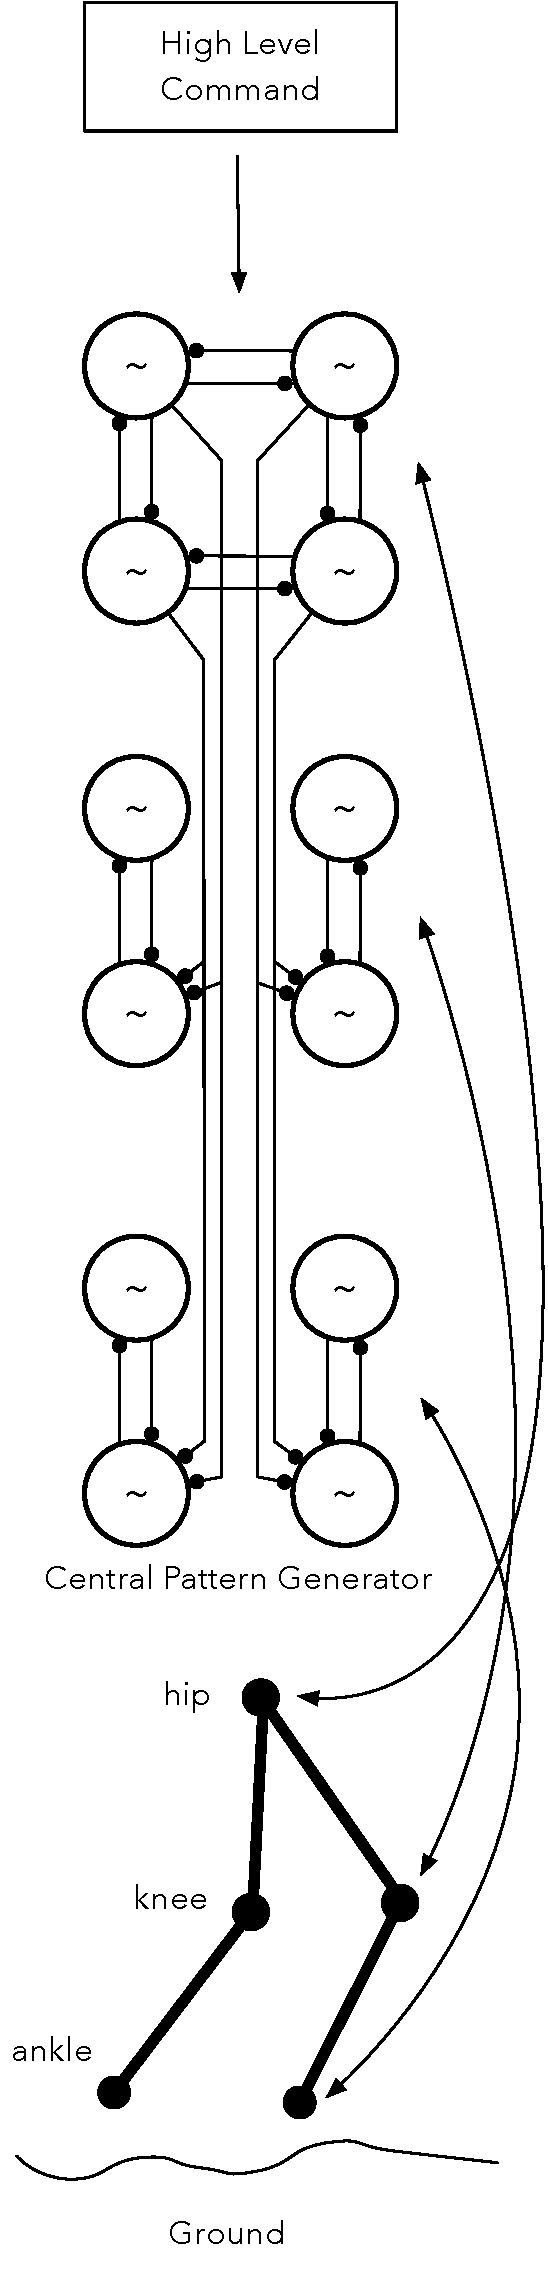
\includegraphics[height=6.25in]{CPG_diagram}
    \caption{Central Pattern Generator for bipedal locomotion as described in
    \citet{taga1991self}. Six neural oscillators receive feedback from and
    command joint torques for the hips, knees, and ankles of a planar biped
    model. A one dimensional high-level control signal enables control of speed
    and elicits gait transitions.}
    \label{fig:cpg_diagram}
\end{marginfigure}
Moreover, research has shown that stimulation of a region of the brain stem
called the Mesencephalic Locomotor Region (MLR) can manipulate the neural
activity generated by CPGs. For example, electrical stimulation of the MLR led
to gait transitions in both decerebrated cats \citep{shik1966control} and
salamanders \citep{cabelguen2003bimodal}.  Therefore, CPGs may serve as a form
of dimensionality reduction and decentralization for the biological control
system as low-dimensional, high-level signals from brain can shape the
high-dimensional, low-level CPG output. Consequently, CPGs may also represent
an attractive option for robotic legged locomotion controllers as
decentralization and dimensionality reduction are desirable properties in this
domain as well.

The seminal work on CPG-based bipedal locomotion control is presented in
\citet{taga1991self}. In this model, a CPG neural network of six interconnected
oscillators describes the joint torques applied to a four link biped model.
Differential equations, first presented in \citet{matsuoka1987mechanisms} with
additional sensory feedback from joint and inertial link angles, describe the
output of the CPG network. The resulting biped model walks with a natural gait
featuring both single and double support and demonstrates robustness to a
variety of disturbances including changes to ground stiffness, damping, and
slope. Additionally, tuning a single parameter induced a transition from walking
to running in the model in a manner comparable to the biological gait
transitions observed after stimulation of the MLR.

CPGs have successfully controlled several bipedal humanoid robots. For example,
\citet{endo2005experimental} used \citeauthor{matsuoka1987mechanisms}'s
nonlinear oscillators along with by bio-inspired feedback pathways that regulate
ground reaction forces and body roll to generate desired foot trajectories for
the bipedal QRIO robot. As in \citeauthor{taga1991self}'s simulations walking
speed can be controlled via adjustment of a single parameter and the robot is
robust to changes in step height. Authors have also succesfully employed other
nonlinear oscillator models. In \citet{shan2002neural}, a Recurrent Neural
Network generates oscillatory signals for a 20-DOF humanoid robot, HOAP-1, that
allow it to walk up and down stairs. In \citet{righetti2006programmable},
programmable ``Hopf'' oscillators \citep{righetti2006dynamic} learn desired
walking trajectories through entrainment enabling HOAP-2, a 25-DOF robot, to
walk forwards and backwards at varying speeds and step lengths.  

CPGs have also been proposed for controlling both mechanically-passive and
active lower limb prostheses.  \citet{nandi2009development} optimize CPG
parameters to fit recorded knee angle trajectories from healthy human subjects.
During walking, the CPG entrains desired knee motions to the oscillations of the
amputee's hip joint. The desired knee angles are achieved in a
mechanically-passive prosthesis via online adjustment of the knee damping.
Similarly, \citet{torrealba2010through, mora2012cybernetic} also use a CPG to
control a mechanically-passive variable damping prosthesis but use phase
resetting to synchronize the amputee and CPG dynamics. 

For active prostheses, \citet{geng2012design} suggest using a Hopf oscillators
to fit the trajectory of the knee angle during walking. \citet{guo2010study}
extend the idea of using a CPG for active prosthesis control by proposing a
hierarchical approach with a support vector machine (SVM) at the high-level
inferring amputee intent from EMG signals, and a CPG at the lower-level
determining the desired knee and ankle angles for an active transfemoral
prosthesis. However, in both cases, the authors do not provide experimental
results on real prosthesis hardware. Moreover, unlike in
\citeauthor{taga1991self}'s original work, these proposed CPG networks for
prostheses generate desired joint kinematics instead of torques. Consequently,
these controllers may not allow prostheses to exhibit the dynamism and
compliance we desire.

\begin{comment}
There exists many models of CPGs of varying complexity: from sub-neural level
models that simulate how ion transport influences signal generation
\citep{hellgren1992computer, traven1993computer} to neuron level models that
investigate how the topology of neuron networks governs rhythmic activity
\citep{buchanan1992neural, williams1992phase}, to high-level models that examine
the role of interconnections between pools of neurons
\citep{matsuoka1987mechanisms, cohen1982nature}.
\citeauthor{matsuoka1987mechanisms}'s model is especially interesting as
\citet{taga1991self} uses this CPG architecture to achieve robust biped
locomotion in simulation. 
\end{comment}

\subsubsection{Reflexes}
Around the same time \citeauthor{brown1911intrinsic} hypothesized the existence
of central pattern generators, \citet{sherrington1910integrative,
sherrington1910flexion} suggested another mechanism for oscillatory neural
signals: chains of reflexes that trigger in response and entrain to sensory
signals. \citeauthor{sherrington1910integrative} identified complex,
multi-joint, multi-limb reflex arcs involving both excitation and inhibition in
response to cutaneous stimulation in decerebrated cats. Moreover, he observed
rhythmic stepping behavior in decerebrated cats suspended off the ground and
concluded that the behavior emerged reflexively based on proprioceptive signals
emanating from the muscles themselves.

In animal experiments discussed earlier, while CPGs can go a long way towards
explaining locomotion neural activity, they still do not fully explain all
observed phenomena. Reflexes or local feedback loops, likely at least shape
locomotion activation patterns through entrainment, for example in Lamprey's
movement of the tail generates activation in the spinal chord of equal frequency
\citep{mcclellan1993mechanosensory} and phase resetting, as demonstrated by the
ability of decerebrated cats to walk on treadmills across a range of speeds
\citep{rossignol2000locomotion}.

For human and primate bipedal locomotion, the roll of CPGs is more muddied and
the roll of reflexes more evident than for decerebrated cats and simpler
vertebrate animals \citep{mackay2002central, vaughan2003theories,
nielsen2003we}. This is perhaps due to the demands of controlling the inherently
unstable dynamics of upright walking \citep{capaday2002special}. For example,
while rhythmic spinal activity has been observed in humans, it is not clear if
the neural signals are an example of autonomous fictive motion, indicative of a
CPG, or entrainment with stretch reflexes in leg muscles
\citep{capaday2002special, stewart1991modulation}. In this case, we can also
look to robotics to provide insight about biology: in the previously discussed
experiments on humanoid robots controlled by CPGs, a significant reduction in
robustness was observed after blocking sensory feedback pathways
\citep{endo2005experimental, righetti2006programmable} indicating CPGs alone may
not fully explain bipedal locomotion. Whereas research has not yet clearly
established the presence of a CPG driving human locomotion, research has
identified many reflexes that contribute to locomotion such as the Hoffman
reflex (H-reflex) of the soleus ankle plantarflexor muscle
\citep{capaday1987difference}, stretch reflex in the soleus
\citep{yang1991contribution}, soleus force feedback \citep{grey2007positive},
and cutaneous reflexes that induce withdrawal responses \citep{yang1990phase}. 

To model the potential interplay between muscular reflexes and CPGs in human
locomotion \citet{ogihara2001generation} and extend the model presented in
\citet{taga1991self} by adding muscles stimulated by alpha motor neurons.  This
model simulates nine muscles of the leg, each stimulated by an alpha motor
neuron that receives input from a CPG oscillator and feedback from
proprioceptive sensors on the muscles.

Whereas models have robot experiments have shown reflexes are vital for
maintaining bipedal gait stability, the came cannot be said about CPGs. In fact,
as shown by \citet{}, it is possible to achieve robust and human-like bipedal
locomotion using only reflexes.

Reflexes in robotics and prosthetics.

\section{Neuromuscular Model}

\subsection{Hill muscle models}
\subsection{Hypothesized Reflexes}
\subsection{Swing Leg Control}
\subsection{Previous results}
\subsubsection{Biped simulations}
    \begin{itemize}
        \item Neuromuscular models replicate characteristics of human walking
        \begin{itemize}
            \item kinematics
            \item emg
            \item kinetics
            \item robust
        \end{itemize}

        \item have been used in animation
    \end{itemize}

\subsubsection{prostheses}
    Has been used in Ankle prosthesis and showed automatic adaptations to slopes
    unlike impedance control which needed retuning


\section{Design of Dynamic Walking Machines}

\subsection{Early Hopping Robots}
\subsubsection{CMU hydraulic six legged}
\subsubsection{Raibert's machines}

\subsection{Bipedal Robots}
\subsubsection{Mabel}
\subsubsection{Atrias}

\subsection{Prostheses}
\subsubsection{Vanderbilt's prostheses}
    \begin{description}
        \item[gen 1] Monopropellant based transfemoral prosthesis
        \item[gen 2] \phantom{text} ~\\
        \begin{itemize}
                \item maxon motors
                \item ball screw transmission
                \item parallel spring in ankle
                \item load cells to measure torque.
            \end{itemize}
        \item[gen 3] ~\\
            \begin{itemize}
                \item maxon flat motors
                \item custom spur gear transmission - high gear ratio
                \item torque sensing ?
            \end{itemize}
        \item[gen 4] ~|\
            \begin{itemize}
                \item maxon flat motors
                \item custom spur gear transmission - high gear ratio
                \item torque sensing ?
            \end{itemize}
    \end{description}
\subsubsection{Hugh Herr's prostheses}
    \begin{description}
        \item[rheo knee]
        \item[biom ankle]
        \item[antagonistic knee]
        \item[CSEA knee]
    \end{description}
